\chapter{UNIQUE HARDWARE CHARACTERISTICS OF A MOBILE DEVICE}\label{cha:character}\index{characteristics}
In the hardware of a device there are some features that can be used to distinguish devices from each other. In most cases it is not called features rather error sources. In the aim of this thesis it is feature characteristics that can be seen as an uniqueness of an mobile device. \textit{Device fingerprint(ing)}\index{device fingerprint} is the term used for this feature characteristics and the pyramid seen in figure~\ref{fig:pyramid} from ~\cite[]{sensor:acoustic} shows the different types of sources of device fingerprint. This thesis will focus on the top of quarter of that pyramid, that is the sensors. All error sources of sensors comes in form of bias and the bias from each sensor covered by the thesis is further explained in this chapter. There is also an explanation on how the sensors is measured from Android respective JavaScript depending on the preformed tests that is described in ~\chapterref{cha:test}.

\begin{figure}[!h]
		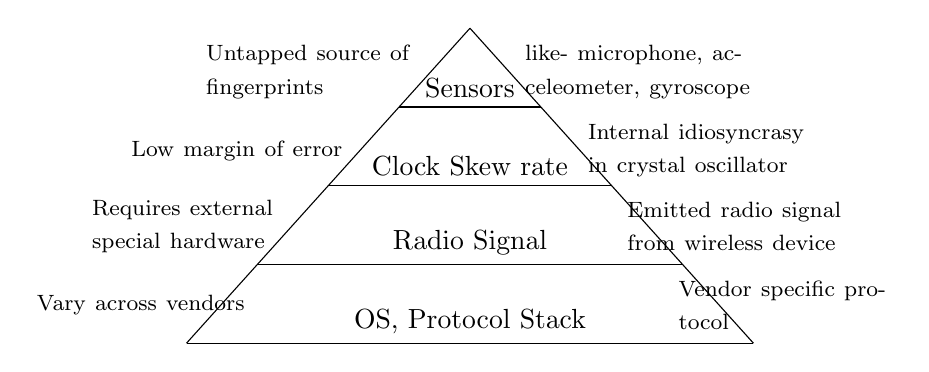
\begin{tikzpicture}[scale=1]

		\def \h {4};
		\def \f {0.9};

		\foreach \y in  {0,1,2,3} {
		    \def \w { \h*\f-\y*\f };
		    \def \v { \y*\f-\h*\f };
		    \draw (\v,\y) -- (\w,\y);
		}

		\draw (-\h*\f,0)  -- (0,\h);
		\draw (\h*\f,0)  -- (0,\h);
		\node (os) at (0,0) [above] {OS, Protocol Stack};
		\node (rf) at (0,1) [above] {Radio Signal};
		\node (cs) at (0,2) [above] {Clock Skew rate};
		\node (se) at (0,3) [above] {Sensors};


		\node [left of=os, xshift=-3cm, yshift=0.2cm, text width=3cm] {\footnotesize{Vary across vendors}};
		\node [left of=rf, xshift=-2.4cm, yshift=0.2cm, text width=2.8cm] {\footnotesize{Requires external special hardware}};
		\node [left of=cs, xshift=-1.8cm, yshift=0.2cm, text width=3cm] {\footnotesize{Low margin of error}};
		\node [left of=se, xshift=-1cm, yshift=0.2cm, text width=2.7cm] {\footnotesize{Untapped source of fingerprints}};

		\node [right of=os, xshift=3cm, yshift=0.2cm, text width=2.7cm] {\footnotesize{Vendor specific protocol}};
		\node [right of=rf, xshift=2.5cm, yshift=0.2cm, text width=3cm] {\footnotesize{Emitted radio signal from wireless device}};
		\node [right of=cs, xshift=2cm, yshift=0.2cm, text width=3cm] {\footnotesize{Internal idiosyncrasy in crystal oscillator}};
		\node [right of=se, xshift=1.2cm, yshift=0.2cm, text width=3cm] {\footnotesize{like- microphone, acceleometer, gyroscope}};
	\end{tikzpicture}
	\caption{\label{fig:pyramid} The pyramid of features in a mobile device that can be used for fingerprinting.\cite[]{sensor:acoustic}}
\end{figure}

As seen above in~\figureref{fig:pyramid} are sensors an untapped source of fingerprints in mobile devices and example of sensors are microphone, accelerometer, barometer, speakers and gyroscope. The sensors investigated in this work is the accelerometer-, gyroscope-, magnetometer- and camera- sensors. All of them are common sensors in most of the mobile devices used today.


\section{Accelerometer\index{accelerometer}}\label{sec:accelerometer}
The accelerometer is the sensor that detect movement on a mobile device, like when you changing orientation on your device. Acceleration is measured by sensing how much pressure the device has in terms of force. The type of accelerometer sensor found in a mobile device is a micro-electromechanical systems known as MEMS sensor. \cite[]{sensors:fusion}
\subsection{Fingerprinting feature / Bias}
Measure the characteristics from the accelerometer is done by taking the long term average of the output when the accelerometer is in rest. That is the biggest error source in the accelerometer and it grows quadratically over time, but when the accelerometer is in rest the error $\epsilon$ can be calculated as a function of time $t$;
$$s(t)=\epsilon * \frac{t^2}{2} $$
\cite[]{sensor:inertialNav}\cite[]{sensors:fusion}


\subsection{Gyroscope\index{gyroscope}}\label{sec:gyroscope}
The gyroscope is sensing how the device is moving in terms of angles, for maintaining or measure the orientation. This is originally  a mechanical system based on the principle of conservation of angular momentum. The most popular Gyroscope for devices today is a MEMS that is using silicon micro-mechanical techniques. Coriolis effect is measured with vibrating elements in the MEMS gyroscope. Coriolis effect is a change of moving objects direction when looking at it from a rotating reference system. The difference from the accelerometer is that the gyroscope measures relative to the device body rather than relative to earth. The equations of Coriolis force;  
$$\boldsymbol{ F}_C = -2 \, m \, (\omega *  v)$$
Where $m$ is the mass of the particle, $\omega$ the angular velocity and $v$ the velocity of the particle in the rotating system. 
\cite[]{sensor:inertialNav}
\subsection{Fingerprinting feature / Bias}
The gyroscope has some error characteristics like constant bias, white noise, bias instability, calibration error and temperature effects. One of these error characteristics that can be tested by reading the output from a gyroscope in rest is the \\\textit{constant bias}\index{constant bias}. That is bias of the gyroscope output when not having any rotation on it. This constant error $\epsilon$ of the bias over time $t$ leads to an angular error that grows linear; 
$$\theta (t)= \epsilon * t $$
If take the long term average output from the gyro in rest, the constant error of a rate gyro can be estimated.\cite[]{sensors:fusion}


\section{Magnetometer\index{magnetometer}}
The magnetometer was originally used for navigation and tracking. The type found in mobile devices is like accelerometer and gyroscope a MEMS sensor. They are known as e-compasses gaussmeters that is measuring of magnetic fields larger than 1 nT.
~\cite{sensor:magn}
\subsection{Fingerprinting feature / Bias}
The two main error sources from measurements of magnetometer are magnetic contamination in the sensor. One of those is iron containing material on the operator and in the instrument and the other one is errors made in the measurements of the frequency. Another type of error is generated if the devices is rotated while the measurements are made. \cite[]{sensors:fusion}

\subsection{Camera}\label{sec:char:camera}\index{camera fingerprinting}\index{camera}
The digital camera of a mobile device also includes sensors and other hardware that can be used as fingerprinting characteristics. The basic is that light travels trough a lens and hits a imaging sensor which contains pixels that has a filter array in front. The filter is for gives each pixel a detected color. The pixels is then put together again to a resulting signal which is send to some final post processing (color correction, white balance, etc.) steps before the image is written to the memory card. In this process there are different kind of noise that effects the image;
\begin{itemize}
	\item[] \textit{\index{shot noise}Shot noise -} the amount of photons hitting the sensor and each pixel varies a random amount
	\item[] \textit{\index{fixed pattern noise}Fixed pattern noise - }there is a small electric current that leaks from photo-diodes in each pixel, caused by dark current
	\item[] \textit{\index{photo-response non-uniformity noise}\index{PRNU}Photo-response non-uniformity noise (PRNU) -} is a noise that is not affected by temperature or humidity. When manufacturing sensors the silicon gets imperfection which causes that pixels aren't equally sensitive to light. This is the main source of pattern noise and makes it really unlikely for two cameras to have the same pattern.
\end{itemize}
The three types of noise can be described as a mathematical model for getting the output of the sensor $y_{ij}$:
$$y_{ij}=f_{ij}(x_{ij}+\eta_{ij})+c_{ij}+\epsilon_{ij}$$
where $f_{ij}$ is a multiple factor close to one that captures PRNU noise, $x_{ij}$ is the number of photons hitting the sensor, $\eta_{ij}$ the shot noise, $c_{ij}$ the dark current and $\epsilon_{ij}$ the additive random noise. The key for a unique fingerprint of the camera (in the mobile device) is to finding $f$.
\cite[]{sensor:camera:DCIdent}


\section{Measurements of sensors on mobile devices}
Measurements of sensors from mobile devices can be gather in different ways. In the work of this thesis two approaches where used by the browser application and by an Android application. The camera is an exception where pictures provides the sensor characteristics.
\begin{figure}[H]
	\centering
    \includegraphics[scale=0.2]{img/device-axes}
    \caption{The coordinate system used for both Android and JavaScript\cite[]{sensor:DeviceOrientation:spec}}
  \label{fig:device-axes}
\end{figure}

\subsection{Android}
Android sensor framework provides raw data with high precision from sensor that are built in the device such as different motions sensors (including accelerometer and gyroscope), environmental sensors and position sensors (e.g. magnetometer). \cite[]{android:sensor}
Android sensor framework classes that is used for gather sensor data is; 
\begin{itemize}
	\item[] \texttt{SensorManager}, a manager used to access the sensor of the device. 
	\item[] \texttt{Sensor}, representing a sensor
	\item[] \texttt{SensorEvent}, an event from a Sensor such data from the sensor, time-stamp or accuracy
	\item[] \texttt{SensorEventListener}, gets a SensorEvent when a sensor or accuracy has changed 
\end{itemize}


\subsubsection{Accelerometer in Android}
\texttt{TYPE\_ACCELEROMETER} is the hardware measurements that measures the force of acceleration with $m/s^2$ as unit. 
This measurements includes the force of gravity, Android also provide \texttt{TYPE\_LINEAR\_ACCELERATION} that is without gravity but that is a combined hardware and software sensor. 

\subsubsection{Gyroscope in Android}

\subsubsection{Fingerprinting in Android}


\subsection{JavaScript}
\end{figure}
\begin{figure}[H]
  \hspace{-2cm}
  \centering
  \begin{minipage}[c]{.23\textwidth}
    \centering
    \includegraphics[scale=0.2]{img/device-alpha}
  \end{minipage}
  \hspace{1.5cm}
  \begin{minipage}[c]{.23\textwidth}
    \centering
    \includegraphics[scale=0.2]{img/device-beta}
  \end{minipage}
  \hspace{1.5cm}
  \begin{minipage}[c]{.23\textwidth}
    \centering
    \includegraphics[scale=0.2]{img/device-gamma}
    \hspace{1cm}
  \end{minipage}
  \caption{The device axes for the JavaScript \texttt{DeviceOrientation} and \texttt{DeviceMotion}}
  \label{fig:device-rot}
\end{figure}

\subsubsection{Accelerometer in JavaScript}
To access the accelerometer data in JavaScript no permission is needed, thus the user do not have to know that the accelerometer is measured. To get measurements from the accelerometer an event listener called \texttt{devicemotion} is added. The output from measurements is the acceleration force in $m/s^2$ according to x-, y- and z-axes as in~\figureref{fig:device-axes} below. 

In JavaScript there are two types of acceleration, \texttt{accelerationIncludingGravity} and \texttt{acceleration}.\texttt{accelerationIncludingGravity} is acceleration made by the device. In context to \texttt{acceleration} not depending on influence of gravity only by the acceleration made on the device. 
The JavaScript for measurements of the accelerometer:
\lstinputlisting{code/acc-listener.js}
\cite[]{sensor:DeviceOrientation:spec}

\subsubsection{Gyroscope in JavaScript}